\documentclass[../main.tex]{memoir}

\begin{document}

\chapter{Relación de Tareas}
\label{sec:tareas}

En la presente sección listamos las tareas que se van a proponer a lo largo de la Unidad Didáctica. Las dividimos en función de su naturaleza: las tareas de explicación se basan en explicaciones que da el profesor sobre los conceptos, procedimientos y actitudes que se deben adquirir; las tareas multimedia o de lectura se basan en la visualización de vídeos aclaratorios y de lecturas y discusiones sobre textos relacionados con la temática (fomentando el hábito de la lectura); las tareas de clase se refieren a actividades propuestas por el profesor y resueltas por el alumno en el aula; y las tareas para casa son aquellas propuestas por el profesor para que el alumno las realice en casa y afiance los conocimientos. Estas dos últimas secciones contienen ejercicios tradicionales y también utilizando recursos tecnológicos.

\section{Tareas de explicación}

\textbf{TE1.} Números complejos. Forma binómica y conjugado. Representación. \\

\textbf{TE2.} Operaciones con números complejos en forma binómica. Implicaciones geométricas. \\

\textbf{TE3.} Forma polar y trigonométrica de un número complejo. Operaciones. \\

\textbf{TE4.} Raíces de una ecuación polinómica. Teorema Fundamental del Álgebra. \\


\section{Tareas multimedia o lectura}

\textbf{TM1.} Visionado del vídeo: \textit{Dimensiones. Números Complejos} \\(https://www.youtube.com/watch?v=eS6uMKx0XP0). \\

\textbf{TM2.} Visionado del vídeo del profesor Chris Budd (University of Bath) que explica la importancia de los números complejos en las redes eléctricas actuales. \\

\textbf{TM3.} Investigación sobre otras aplicaciones de los números complejos en la vida real. Exposición ante los compañeros. \\

\textbf{TL1.} Lectura y discusión de extractos de los libros \cite{argand1971}, \cite{nahin1998}, \cite{blank1999} y \cite{descartes1952}.

\section{Tareas de clase}

\textbf{TCl1.} Representa gráficamente los siguientes números complejos y calcula, posteriormente, sus módulos y argumentos.

\begin{itemize}
	\item $z_1 = 4+4i$
	\item $z_2 = -\sqrt{3}+i$
	\item $z_3=5$
	\item $z_4=-3i$
	\item $z_5 = 2-3i$
\end{itemize}

\textbf{TCl2.} Opera y escribe en forma binómica estos complejos. Utiliza Geogebra para representarlos gráficamente. ¿Qué relaciones observas entre las operaciones y la representación gráfica?

\begin{itemize}
	\item $(1+i)(3-2i)$
	\item $2i (3+4i)$
	\item $\displaystyle\frac{1+i}{i}$
	\item $\displaystyle \frac{2-3i}{4+2i}$
	\item $\displaystyle \frac{2}{1+i} - \frac{3}{1-i}$
	\item $\displaystyle \frac{1}{4+3i} \frac{1+i}{i}$
\end{itemize}

\textbf{TCl3.} Escribe en forma binómica $1+i+i^2+i^3+\dots+i^{100}$ \\


\textbf{TCl4.} Resuelve las operaciones indicadas para los números complejos $z_1=2_{60\degree}, z_2=-1+i, z_3  = 2(\cos 210\degree +i \sin 210\degree)$:
\begin{itemize}
	\item $z_1 z_2 z_3$
	\item $\displaystyle \frac{z_1 \overline{z_2}}{z_3}$
	\item $z_3^4$
	\item $z_2^{-2}$
\end{itemize}

\textbf{TCl5.} Considera el polinomio $P(z) = z^3+(-2+3i)z^2 +(13-i)z-6-10i$. ¿Son los números complejos $i, 3$ y $1+i$ raíces de $P(z)$? \\

\textbf{TCl6.} Encuentra el conjunto de todos los complejos que cumplen la condición dada en cada caso. Representa la región con Geogebra.


\begin{itemize}
	\item \textbf{a)} Re $z \geq$ Im $z$
	\item \textbf{b)} $|z-1+3i| < 4$
	\item \textbf{c)} $|z-3| + |z+3| = 10$
\end{itemize}

\textbf{TCl7.} Resuelve la ecuación $z^3-6z^2+12z-16=0$ \\


\textbf{TCl8.} Definir número complejos en wxMaxima. \\

\textbf{TCl9.} Calcular la forma binómica, parte real, parte imaginaria, módulo y argumento principal de un número complejo en wxMaxima. \\

\textbf{TCl10.} Transformar un número complejo de forma binómica a polar y trigonométrica en wxMaxima. \\

\textbf{TCl11.} Resolver ecuaciones polinómicas con raíces complejas en wxMaxima. \\


\section{Tareas para casa}
\textbf{TC1.}  Sean los números complejos $z_1 = -2+i, z_2=-3-2i, z_3 = -5i, z_4 = 4$.
\begin{itemize}
	\item Represéntalos junto con sus opuestos y sus conjugados (dos en papel, dos en Geogebra).
	\item Halla su módulo y argumento.
	\item Determina el módulo y el argumento de sus opuestos.
	\item Determina el módulo y el argumento de sus conjugados
\end{itemize}

\textbf{TC2.} Usa el plano complejo interactivo de Geogebra siguiente para encontrar parejas de números complejos cuyo producto sea un número real. ¿Qué observas? ¿Puedes explicarlo algebraicamente? Haz lo mismo para obtener números imaginarios puros. \\

En general, ¿por qué número necesitas multiplicar $a+bi$ para obtener un número real? ¿Y un imaginario puro? \\

Para un número complejo $a+bi$ dado, ¿por cuánto necesitarías multiplicar para obtener otro número $x+iy$ dado? ¿Qué conclusiones acerca de la interpretación geométrica de la multiplicación extraes? \\

\begin{figure}[H]
	\centering
	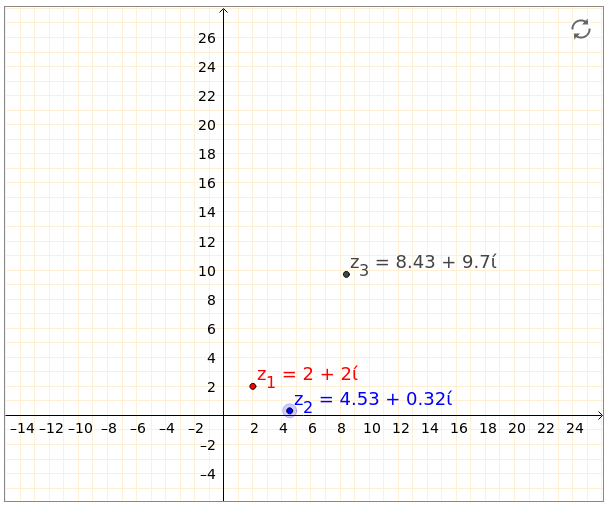
\includegraphics[scale=0.3]{images/geogebra-interactivo.png}
	\caption{Plano complejo interactivo. Geogebra}
	\label{geogebra-interact}
\end{figure}

\textbf{TC3.} Justifica que $(1+i)^8$ es un número real positivo. \\

\textbf{TC4.} Halla todos los números reales $x,y$ tales que $\frac{x+yi}{x-yi}=x-yi$. Expresar en forma polar y trigonométrica $x+yi, x-yi$. \\


\textbf{TC5.} Escribe los siguientes números complejos en forma binómica y forma polar:

\begin{itemize}
	\item \textbf{a)} $2(3-4i)-5(1-i)$
	\item \textbf{b)} $(1-i)(2-i)(3-i)$
	\item \textbf{c)} $(\sqrt{3}+i)^2$
	\item \textbf{d)} $\displaystyle \frac{4+3i}{3-4i}$
	\item \textbf{e)} $\displaystyle \frac{5-z}{5+z}$ siendo $z=4+3i$
\end{itemize}


\textbf{TC6.} ¿Cuántos números complejos $z$ verifican que $z^{2021} = \overline{z}$ \\

\textbf{TC7.} Considera la ecuación $z^2-4z+a=0$ donde $a$ es un número complejo. Determina el valor de $a$ para que el número complejo $2+i$ sea solución de dicha ecuación y, sin hacer ningún cálculo más, escribe la otra solución de dicha ecuación. \\

\textbf{TC8. (Ampliación)} Diseñar y desarrollar una calculadora de números complejos en un lenguaje de programación libre (wxMaxima, Python, C++...).

\newpage

\chapter{Anexo I: Prueba Escrita}

\begin{enumerate}
	\item Expresa en todas sus formas el número complejo que tiene módulo 4 y argumento $120\degree$.
	\item Halla las soluciones complejas de la ecuación $x^4+10x^2+9=0$.
	\item Sea $z=-1+2i$
	\begin{itemize}
		\item Represéntalo y calcula su módulo y las razones trigonométricas de su argumento $\alpha$.
		\item Halla $\tg(\alpha+45\degree), \cos(2\alpha), \sin(2\alpha)$.
		\item Calcula $z^2$ de dos formas distintas expresando el resultado en forma binómica.
		\item Halla $x \in \mathbb{R}$ para que $\frac{x-i}{z}$ sea imaginario puro.
		\item Halla $x \in \mathbb{R}$ para que $z(2+xi)$ tenga su afijo en la bisectriz del 2º al 4º cuadrante.
	\end{itemize}
	\item Calcula y representa todas las soluciones complejas de la ecuación $x^3-8i=0$.
	\item Indica los matemáticos más importantes en el desarrollo de los números complejos y sus aplicaciones actuales.
\end{enumerate}

\end{document}

%%% Local Variables:
%%% mode: latex
%%% TeX-master: "../main"
%%% End:
